%\section{Introduction}

\begin{frame}{Introduction}
    \begin{itemize}[<+->]
        \item Now, we have studied Fourier series and Fourier transform for CT signals.
        \item In this lesson we will develop a similar tool for discrete time.
        \item Specifically, we consider the representation of discrete-time signals through a decomposition as a linear combination of complex exponentials.
            \begin{itemize}
                \item DT periodic signals $\rightarrow$ DT Fourier series
                \item DT aperiodic signals $\rightarrow$ DT Fourier transform
            \end{itemize}
    \end{itemize}
\end{frame}


\begin{frame}{Philosophy}
        \begin{center}
            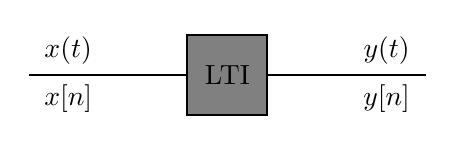
\begin{tikzpicture}
                \draw[thick] (0,0)  -- ++(2,0)node[near start, above] {$x(t)$} node[near start, below] {$x[n]$} node (s) [rectangle, draw=black, thick, fill=gray, minimum width=0.4in, minimum height = 0.4in,anchor=west] {LTI} (s.east) -- ++(2,0) node[near end, above] {$y(t)$} node[near end, below] {$y[n]$};
            \end{tikzpicture}
        \end{center}
        Decompose the input as
            \begin{equation*}
                x = a_1\phi_1 + a_2\phi_2 + \cdots \quad \text{linear combination of basic inputs}
            \end{equation*}
        Then
            \begin{equation*}
                y = a_1\psi_1 + a_2\psi_2 + \cdots \quad \text{linear combination of corresponding outputs}
            \end{equation*}

        Choose $\phi_k(t)$ or $\phi_k[n]$ such that
        \begin{itemize}
            \item Broad class of signals can be constructed, and
            \item Response to $\phi_k$s easy to compute.
        \end{itemize}
\end{frame}

\begin{frame}{Eigenfunction Property}
    \textbf{Continuous-Time}:\par
    $\phi_k(t) = e^{j\omega_k t}$:
    \begin{equation*}
        e^{j\omega_k t} \longrightarrow H(\omega_k) e^{j\omega_k t} \quad \text{(a scaled-version of the input)}
    \end{equation*}
    \textbf{``Discrete-Time'':}\pause
    \mode<beamer>
    {
        $\phi_k[n] = e^{j\omega_k n}$\par
        \begin{equation*}
            e^{j\omega_k n} \longrightarrow
            \underset{\mathclap{\tikz \node {$\uparrow$} node [below=3ex, text=red] {eigenfunction};}}{
            e^{j\omega_k n}
            }
            \underbrace{
            \sum_{r=-\infty}^{\infty} h[r]e^{-j\omega_k r}
            }_{\textcolor{red}{\text{eigenvalue}}}
        \end{equation*}
    }
\end{frame}




\begin{frame}{Discrete-Time Fourier Series}
    \mode<beamer>
    {
        \begin{columns}
            \column{0.48\textwidth}
                Consider $x[n]$ to be periodic,\par
                Period $N$,\par
                Fundamental frequency $\omega_0 = \frac{2\pi}{N}$\par
                $e^{jk\omega_0 n}$ are harmonically related, and periodic with the period $N$, although the fundamental period is different.
                $e^{jk\omega_0 n} = e^{j(k+N)\omega_0 n}$\par
                \par\pause
                Consider the complex exponential
                \begin{equation*}
                    e^{jk\omega_0n} = e^{j(k+N)\omega_0n}
                \end{equation*}
                $\Rightarrow$ Only $N$ distinct complex exponentials.
            \column{0.48\textwidth}
                \begin{equation*}
                    x[n] = \sum_k a_k e^{jk\omega_0 n}, \quad k = 0,1, 2, \dots, N-1.
                \end{equation*}
                \begin{equation*}
                    x[n] = \sum_{k=<N>} a_k e^{jk\omega_0 n}.
                \end{equation*}
                $N$ equations in $N$ unknowns.
                \begin{equation*}
                    a_k = \frac{1}{N}\sum_{<N>} x[n]e^{-jk\omega_0 n}.
                \end{equation*}
                $k = <N>$: $k$ ranges over one period (as $a_k$ periodically repeats).
        \end{columns}
    }
\end{frame}


\begin{frame}{Discrete-Time Fourier Series}
    %\mode<beamer>
    %{
        \begin{columns}
            \column{0.48\textwidth}
            \textbf{Continuous-Time}\par
            \begin{align*}
                x(t) &= \sum_{k=-\infty}^{\infty}a_k e^{jk\omega_0 t}\\
                a_k &= \frac{1}{T} \int_{T} x(t)e^{-jk\omega_0 t}dt
            \end{align*}
            \column{0.48\textwidth}

            \textbf{Discrete-Time Fourier Series}
            \mode<beamer>
            {

            \begin{align*}
                \text{Synthesis} &\\
                x[n] &= \sum_{k=<N>} a_k e^{jk\omega_0 n} = \sum_{k=<N>} a_k e^{jk(2\pi/N) n} .\\
                \text{Analysis} &\\
                a_k &= \frac{1}{N}\sum_{n=<N>} x[n]e^{-jk\omega_0 n}  = \frac{1}{N}\sum_{n=<N>} x[n]e^{-jk(2\pi/N) n}.
            \end{align*}
            \pause
            Note the duality.
            }
        \end{columns}
    %}
\end{frame}



\begin{frame}


    \mode<beamer>
    {
        \begin{columns}
            \column{0.48\textwidth}
            \textbf{Periodicity}
                \begin{equation*}
                    \begin{array}{lll}
                        x[n] & \text{periodic in } n, & \text{true for CT}\\
                        e^{jk\omega_0 n} & \text{periodic in } n, &\text{true for CT}\\
                        e^{jk\omega_0 n} & \text{periodic in } k, &\text{\alert{not true for CT}}\\
                        a_k &  \text{periodic in } k, &\text{\alert{not true for CT}}
                    \end{array}
                \end{equation*}
            \column{0.48\textwidth}
            \textbf{Convergence}\par
            Continuous-time:
            \begin{itemize}
                \item $x(t)$ square-integrable OR
                \item Dirichlet condition
            \end{itemize}
            Discrete-time
            \begin{equation*}
                x[n] = \sum_{k=<N>} a_k e^{jk\omega_0 n}.
            \end{equation*}
            \begin{equation*}
                \hat{x}[n] = \sum_{p \text{ terms}} a_k e^{jk\omega_0 n}.
            \end{equation*}
            $p = N$\par
            \begin{equation*}
                \hat{x}[n] \equiv x[n].
            \end{equation*}
            There is no issue of convergence in DT.
        \end{columns}
    }
\end{frame}

\begin{frame}
    \begin{example}
        Consider the signal
        \begin{enumerate}
            \item When is this signal periodic?
            \item If it is periodic, what are discrete-time Fourier series coefficients?
        \end{enumerate}
    \end{example}
    \pause
    \mode<beamer>
    {
        This is the DT counterpart of $x(t) = \sin \omega_0 t$. $x[n]$ is periodic only if $2\pi/\omega_0$ is an integer or a ratio of integers. For the case when $2\pi/\omega_0$ is an integer $N$, i.e., when
        \begin{equation*}
            \omega_0 = \frac{2\pi}{N},
        \end{equation*}
        $x[n]$ is periodic with fundamental period $N$.
    }
    \pause
    \mode<beamer>
    {
        Expanding the signal as a sum of two complex exponentials,
        \begin{equation}
            x[n] = \frac{1}{2j}e^{j(2\pi/N)n} - \frac{1}{2j}e^{-j(2\pi/N)n}.
        \end{equation}
        \pause
        \begin{equation*}
            a_1 = \frac{1}{2j}, \quad a_{-1} = -\frac{1}{2j}.
        \end{equation*}
    }

\end{frame}

\begin{frame}{Fourier Coefficients for $x[n] = \sin(2\pi/N)n$ for $N=5$ }
    \begin{figure}
        \centering
        \begin{filecontents}{sinomega.dat}
o reak akmag imak argak
-11 -0.5 0 0 0
-10 0 0 0 0 
-9 0.5 0 0 0 
-8 0 0 0 0
-7 0 0 0 0
-6 -0.5 0 0 0
-5 0 0 0 0
-4 0.5 0 0 0
-3 0 0 0 0
-2 0 0.5 -0.5 -1.57
-1 -0.5 1.581 0.5 0.32
0  0 1 0 0
1 0.5 1.581 -0.5 -0.32
2 0 0.5 0.5 1.57
3 0 0 0 0
4 -0.5 0 0 0
5 0 0 0 0
6 0.5 0 0 0
7 0 0 0 0
8 0 0.5 -0.5 -1.57
9 -0.5 0 0 0
10  0 0 0 0
11 0.5 0 0 0
\end{filecontents}
\pgfplotstableread{sinomega.dat}{\sinomega}

\begin{tikzpicture}[scale=0.6]



    \begin{axis}[
    		name=axis1,
% 		y=1cm,
 		x=0.7cm,
		 clip=false,
		 xmin=-12,xmax=12,
		 xlabel= $k$,
		 ylabel={$a_k$},
		 ymin=-1,ymax=1,
		axis lines=middle,
         	xtick={-11, -10, ..., 11},
         	%xticklabels={$-N$, $0$, $N$},
		 ytick={-1, 1},
		 yticklabels=\empty,
		 every axis x label/.style={at={(ticklabel* cs:1.05)}, anchor=west,},
		every axis y label/.style={at={(ticklabel* cs:1.05)}, anchor=south,},
     ]
	\addplot [red,very thick, ycomb] table [x={o}, y={reak}] {\sinomega};
	\node at (axis cs:-1,-0.5) [anchor= east] {\small $-\dfrac{1}{2j}$};
	\node at (axis cs:1,.5) [anchor= west] {\small $\dfrac{1}{2j}$};	
	\end{axis}
			
\end{tikzpicture} 
        \caption{Fourier coefficients for $x[n] = \sin(2\pi/5)n$.}
    \end{figure}
\end{frame}

\begin{frame}{Example}
    Determine and sketch the DTFS of
    \begin{equation*}
        x[n] = 1 + \sin \omega_0 n + 3 \cos \omega_0 n + \cos\left(2\omega_0 n + \frac{\pi}{2}\right).
    \end{equation*}
    \pause
\end{frame}

\begin{frame}
    \begin{figure}
        \centering
        \begin{filecontents}{example52data.dat}
o reak akmag imak argak
-15 0 0 0 0
-14 0 0 0 0
-13 0 0 0 0
-12 0 0.5 -0.5 -1.57
-11 1.5 1.581 0.5 0.32
-10 1 1 0 0
-9 1.5 1.581 -0.5 -0.32
-8 0 0.5 0.5 1.57
-7 0 0 0 0
-6 0 0 0 0
-5 0 0 0 0
-4 0 0 0 0
-3 0 0 0 0
-2 0 0.5 -0.5 -1.57
-1 1.5 1.581 0.5 0.32
0  1 1 0 0
1 1.5 1.581 -0.5 -0.32
2 0 0.5 0.5 1.57
3 0 0 0 0
4 0 0 0 0
5 0 0 0 0
6 0 0 0 0
7 0 0 0 0
8 0 0.5 -0.5 -1.57
9 1.5 1.581 0.5 0.32
10  1 1 0 0
11 1.5 1.581 -0.5 -0.32
12 0 0.5 0.5 1.57
13 0 0 0 0
14 0 0 0 0
15 0 0 0 0
\end{filecontents}
\pgfplotstableread{example52data.dat}{\ninivina}

\begin{tikzpicture}[scale=0.6]	



    \begin{axis}[
    		name=axis1,
% 		y=1cm,
% 		x=1cm,
		 clip=false,
		 xmin=-12,xmax=12,
		 xlabel= $k$,
		 ylabel={$\mathfrak{Re}\{a_k\}$},
		 ymin=-1.5,ymax=2,
		axis lines=middle,
         	xtick={-10, 0, 10},
         	xticklabels={$-N$, $0$, $N$},
		 ytick={-1, 1},
		 yticklabels=\empty,
		 every axis x label/.style={at={(ticklabel* cs:1.05)}, anchor=west,},
		every axis y label/.style={at={(ticklabel* cs:1.05)}, anchor=south,},
     ]
	\addplot [red,very thick, ycomb] table [x={o}, y={reak}] {\ninivina};
	\node at (axis cs:0,1) [anchor= west] {\small $1$};
	\node at (axis cs:1,1.5) [anchor= west] {\small $\dfrac{3}{2}$};	
	\end{axis}
	
    \begin{axis}[
    		name=axis2,
    		at={($(axis1.east)+(10cm,0)$)},anchor= east,
% 		y=1cm,
% 		x=1cm,
		 clip=false,
		 xmin=-12,xmax=12,
		 xlabel= $k$,
		 ylabel={$|a_k|$},
		 ymin=-1.5,ymax=2,
		axis lines=middle,
         	xtick={-10, 0, 10},
         	xticklabels={$-N$, $0$, $N$},
		 ytick={-1, 1},
		 yticklabels=\empty,
		 every axis x label/.style={at={(ticklabel* cs:1.05)}, anchor=west,},
		every axis y label/.style={at={(ticklabel* cs:1.05)}, anchor=south,},
     ]
	\addplot [red,very thick, ycomb] table [x={o}, y={akmag}] {\ninivina};
	\node at (axis cs:0,1) [anchor= west] {\small $1$};
	\node at (axis cs:1,1.5) [anchor= west] {\small $\dfrac{\sqrt{10}}{2}$};		
	\node at (axis cs:2,.5) [anchor= west] {\small $\dfrac{1}{2}$};			
	\end{axis}	
	
    \begin{axis}[
    		name=axis3,
    		at={($(axis1.south east)+(0,-1.1cm)$)},anchor=north east,
% 		y=1cm,
% 		x=1cm,
		 clip=false,
		 xmin=-12,xmax=12,
		 xlabel= $k$,
		 ylabel={$\mathfrak{Im}\{a_k\}$},
		 ymin=-1.5,ymax=2,
		axis lines=middle,
         	xtick={-10, 0, 10},
         	xticklabels={$-N$, $0$, $N$},
		 ytick={-1, 1},
		 yticklabels=\empty,
		 every axis x label/.style={at={(ticklabel* cs:1.05)}, anchor=west,},
		every axis y label/.style={at={(ticklabel* cs:1.05)}, anchor=south,},
     ]
	\addplot [red,very thick, ycomb] table [x={o}, y={imak}] {\ninivina};
	\node at (axis cs:-1,.5) [anchor= east] {\small $\dfrac{1}{2}$};
	\node at (axis cs:1,-.5) [anchor= west] {\small $-\dfrac{1}{2}$};
	\end{axis}	
	
    \begin{axis}[
    		name=axis4,
    		at={($(axis2.south east)+(0,-1.1cm)$)},anchor=north east,
% 		y=1cm,
% 		x=1cm,
		 clip=false,
		 xmin=-12,xmax=12,
		 xlabel= $k$,
		 ylabel={$\angle a_k$},
		 ymin=-1.5,ymax=2,
		axis lines=middle,
         	xtick={-10, 0, 10},
         	xticklabels={$-N$, $0$, $N$},
		 ytick={-1, 1},
		 yticklabels=\empty,
		 every axis x label/.style={at={(ticklabel* cs:1.05)}, anchor=west,},
		every axis y label/.style={at={(ticklabel* cs:1.05)}, anchor=south,},
     ]
	\addplot [red,very thick, ycomb] table [x={o}, y={argak}] {\ninivina};
	\node at (axis cs:2,1.5) [anchor= west] {\small $\dfrac{\pi}{2}$};
	\node at (axis cs:-2,-1.5) [anchor= east] {\small $-\dfrac{\pi}{2}$};	
	\end{axis}		
\end{tikzpicture} 
    \end{figure}
\end{frame}

\begin{frame}{Example}
    Determine and sketch the DTFS of $x[n]$ of which is shown in the figure.
    \begin{figure}
        \centering
        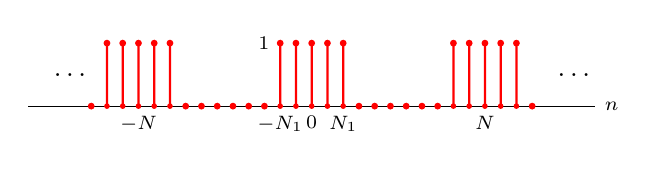
\begin{tikzpicture}[scale=0.8]

	\def\nmin{-13}
	\def\nmax{13}	
	
	\begin{scope}	
		\def\x{{0, 1, 1, 1, 1, 1, 0, 0, 0, 0, 0, 0, 1, 1, 1, 1, 1, 0, 0, 0, 0, 0, 0, 1, 1, 1, 1, 1, 0}}	

		\draw (-4.25, 0) -- (4.75, 0) node[anchor=west] {\scriptsize $n$};
		\foreach \n/\l in {-10/{-N}, -1/{-N_1}, 1/0, 3/{N_1}, 12/{N}}
		{
			\node at (\n/4, 0) [anchor=north] {\scriptsize $\l$};
		}
		\node at (-0.75,1) [anchor=west] {\scriptsize $1$};
		\node at (4,0.5) [anchor=west] {$\dots$};
		\node at (-4,0.5) [anchor=west] {$\dots$};
		
		\foreach \n in {0,1, ..., 28}
		{
			\pgfmathparse{\x[\n]}
			\edef\xn{\pgfmathresult}	
			\ifthenelse{\xn > 0}
			{
				\draw[red, thick, fill=red]  (\n/4 + \nmin/4, 0) -- ++(0, \xn) circle (1pt);% node[anchor=east] {\scriptsize $\xn$};
			}
			{
				\draw[red, fill=red] (\n/4+ \nmin/4,  0) circle (1pt);
			}
		}
	\end{scope}	
\end{tikzpicture}
    \end{figure}
    \pause
\end{frame}


\begin{frame}
    \mode<beamer>
    {
        \begin{align*}
                a_k &= \frac{1}{N}\sum_{n=-N_1}^{N_1}e^{-jk(2\pi/N)n}\\
                \text{Letting~} m = n+N_1&\pause\\
                &= \frac{1}{N}\sum_{m=0}^{2N_1}e^{-jk(2\pi/N)/(m- N_1)}\\
                2N_1 + 1\text{~terms in a geometric series}&\\
                &= \frac{1}{N}e^{jk(2\pi/N)N_1}\left[\frac{1 - e^{-jk(2\pi/N)(2N_1 + 1)}}{1 - e^{-jk(2\pi/N)}}\right]\pause\\
                &=  \frac{1}{N} e^{jk(2\pi/N)N_1} \cdot
                \frac{
                    e^{-j\frac{k(2\pi/N)(2N_1+1)}{2}}
                }{
                e^{-j\frac{k(2\pi/N)}{2}}
                } \left[
                \frac{e^{j\frac{k(2\pi/N)(2N_1+1)}{2}}  - e^{-j\frac{k(2\pi/N)(2N_1+1)}{2}} }
                {e^{j\frac{k(2\pi/N)}{2}} - e^{-j\frac{k(2\pi/N)}{2}}}\right]\pause\\
                &=  \frac{1}{N} \frac{\sin\left[ \frac{k(2\pi/N)(2N_1+1)}{2} \right]}{\sin\left[\frac{k(2\pi/N)}{2}\right]}\pause\\
        \end{align*}
    }
\end{frame}

\begin{frame}
    \mode<beamer>
    {
        \begin{align*}
                a_k &=  \frac{1}{N} \frac{\sin\left[ 2\pi k(N_1+1/2)/N \right]}{\sin(\pi k/N)}\quad k \neq 0, \pm N, \pm 2N, \dots\\
                a_k &= \frac{2N_1+1}{N}\quad k = 0, \pm N, \pm 2N, \dots.
        \end{align*}
    }
\end{frame}

\begin{frame}
    \begin{figure}
        \centering
        \begin{tikzpicture}[scale=0.3]	


    \begin{axis}[
    		name=axis1,
		y=1cm,
		x=1cm,
		 clip=false,
		 xmin=-3.5,xmax=10,
		 xlabel= $\omega$,
		 ylabel={$Na_k$},
		 ymin=-1.5,ymax=6,
		 axis lines=middle,
         	xtick={-3.1416, 3.1416, 6.2832},
         	xticklabels={$-\pi$, $\pi$, $2\pi$},
		 %ytick={-1, 1},
		 yticklabels=\empty,
		 every axis x label/.style={at={(ticklabel* cs:1.05)}, anchor=west,},
		every axis y label/.style={at={(ticklabel* cs:1.05)}, anchor=south,},
     ]
		\addplot [red, smooth, mark=none] table [x={o}, y={xo}] {g_dt_fs/figures/dtfs_square_N10.dat};
		\addplot [blue, ycomb, mark=*] table [x={o}, y={xo}] {g_dt_fs/figures/dtfs_square_stem_N10.dat};

		\node at (axis cs:10, 3) [anchor=east] { $N=10$ };
    \end{axis}


\pause
    \begin{axis}[
    	name=axis2,
    	at={($(axis1.south east)+(0,-1.1cm)$)},anchor=north east,
		y=1cm,
		x=1cm,
		 clip=false,
		 xmin=-3.5,xmax=10,
		 xlabel= $\omega$,
		 ylabel={$Na_k$},
		 ymin=-1.5,ymax=6,
		 axis lines=middle,
         	xtick={-3.1416, 3.1416, 6.2832},
         	xticklabels={$-\pi$, $\pi$, $2\pi$},
		 %ytick={-1, 1},
		 yticklabels=\empty,
		 every axis x label/.style={at={(ticklabel* cs:1.05)}, anchor=west,},
		every axis y label/.style={at={(ticklabel* cs:1.05)}, anchor=south,},
     ]
		\addplot [red, smooth, mark=none] table [x={o}, y={xo}] {g_dt_fs/figures/dtfs_square_N20.dat};%.
		\addplot [blue, ycomb, mark=*] table [x={o}, y={xo}] {g_dt_fs/figures/dtfs_square_stem_N20.dat};%.

		\node at (axis cs:10, 3) [anchor=east] { $N=20$ };
    \end{axis}

\pause
        \begin{axis}[
    	name=axis3,
    	at={($(axis2.south east)+(0,-1.1cm)$)},anchor=north east,
		y=1cm,
		x=1cm,
		 clip=false,
		 xmin=-3.5,xmax=10,
		 xlabel= $\omega$,
		 ylabel={$Na_k$},
		 ymin=-1.5,ymax=6,
		 axis lines=middle,
         	xtick={-3.1416, 3.1416, 6.2832},
         	xticklabels={$-\pi$, $\pi$, $2\pi$},
		 %ytick={-1, 1},
		 yticklabels=\empty,
		 every axis x label/.style={at={(ticklabel* cs:1.05)}, anchor=west,},
		every axis y label/.style={at={(ticklabel* cs:1.05)}, anchor=south,},
     ]
		\addplot [red, smooth, mark=none] table [x={o}, y={xo}] {g_dt_fs/figures/dtfs_square_N40.dat};
		\addplot [blue, ycomb, mark=*] table [x={o}, y={xo}] {g_dt_fs/figures/dtfs_square_stem_N40.dat};

		\node at (axis cs:10, 3) [anchor=east] { $N=40$ };
    \end{axis}

\end{tikzpicture} 
    \end{figure}
\end{frame}



\section{Properties of Discrete-Time Fourier Series}


\begin{frame}{Example}
    Find the Fourier series coefficients $a_k$ of $x[n]$.
    \begin{figure}
        \centering
        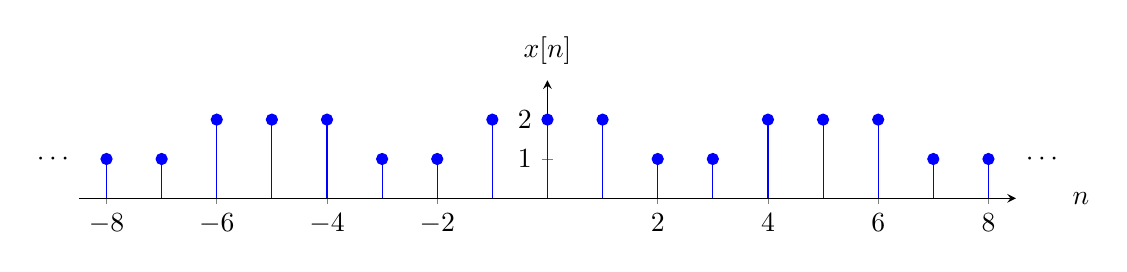
\begin{tikzpicture}[scale=1]	


\begin{filecontents}{example313.dat}
o    xo
-8 1
-7 1
-6 2
-5 2
-4 2
-3 1
-2 1
-1 2
0 2
1 2
2 1
3 1
4 2
5 2
6 2
7 1
8 1
\end{filecontents}

    \begin{axis}[
    		name=axis1,
		y=0.5cm,
		x=0.7cm,
		 clip=false,
		 xmin=-8.5,xmax=8.5,
		 xlabel= $n$,
		 ylabel={$x[n]$},
		 ymin=0,ymax=3,
		 axis lines=middle,
         %xtick={-3.1416, -2.513, -1.885, -1.257, -0.6283, 0, 0.6283, 1.257, 1.885, 2.513, 3.1416, 6.2832},
         %xticklabels={-5, -4, -3, -2, -1, 0, 1, 2, 3, 4, 5, 10 },
		 ytick={1, 2},
		 yticklabels={1,2},
		 every axis x label/.style={at={(ticklabel* cs:1.05)}, anchor=west,},
		every axis y label/.style={at={(ticklabel* cs:1.05)}, anchor=south,},
     ]
		%\addplot [red, smooth, mark=none] table [x={o}, y={xo}] {example313.dat;%
		\addplot [blue, ycomb, mark=*] table [x={o}, y={xo}] {example313.dat};%

		\node at (axis cs:8.5, 1) [anchor=west] { $\cdots$ };
		\node at (axis cs:-8.5, 1) [anchor=east] { $\cdots$ };		
    \end{axis}

%
% %\pause
%     \begin{axis}[
%     	name=axis2,
%         	at={($(axis1.south east)+(0,-0.5cm)$)},anchor=north east,
% 		y=0.25cm,
% 		x=0.8cm,
% 		 clip=false,
% 		 xmin=-3.5,xmax=10,
% 		 xlabel= $k$,
% 		 ylabel={$Na_k$},
% 		 ymin=-1.5,ymax=6,
% 		 axis lines=middle,
%          xtick={-3.1416, -2.513, -1.885, -1.257, -0.6283, 0, 0.6283, 1.257, 1.885, 2.513, 3.1416, 6.2832},
%          xticklabels={-10, -8, -6, -4, -2, 0, 2, 4, 6, 8, 10, 20 },
% 		 %ytick={-1, 1},
% 		 yticklabels=\empty,
% 		 every axis x label/.style={at={(ticklabel* cs:1.05)}, anchor=west,},
% 		every axis y label/.style={at={(ticklabel* cs:1.05)}, anchor=south,},
%      ]
% 		\addplot [red, smooth, mark=none] table [x={o}, y={xo}] {g_dt_fs/figures/dtfs_square_N20.dat};%.
% 		\addplot [blue, ycomb, mark=*] table [x={o}, y={xo}] {g_dt_fs/figures/dtfs_square_stem_N20.dat};%.
%
% 		\node at (axis cs:10, 3) [anchor=east] { $N=20$ };
%     \end{axis}
%
% %\pause
%         \begin{axis}[
%     	name=axis3,
%     	at={($(axis2.south east)+(0,-0.5cm)$)},anchor=north east,
% 		y=0.25cm,
% 		x=0.8cm,
% 		 clip=false,
% 		 xmin=-3.5,xmax=10,
% 		 xlabel= $k$,
% 		 ylabel={$Na_k$},
% 		 ymin=-1.5,ymax=6,
% 		 axis lines=middle,
%          xtick={-3.1416, -2.513, -1.885, -1.257, -0.6283, 0, 0.6283, 1.257, 1.885, 2.513, 3.1416, 6.2832},
%          xticklabels={-20, -16, -12, -8, -4, 0, 4, 8, 12, 16, 20, 40 },
% 		 %ytick={-1, 1},
% 		 yticklabels=\empty,
% 		 every axis x label/.style={at={(ticklabel* cs:1.05)}, anchor=west,},
% 		every axis y label/.style={at={(ticklabel* cs:1.05)}, anchor=south,},
%      ]
% 		\addplot [red, smooth, mark=none] table [x={o}, y={xo}] {g_dt_fs/figures/dtfs_square_N40.dat};
% 		\addplot [blue, ycomb, mark=*] table [x={o}, y={xo}] {g_dt_fs/figures/dtfs_square_stem_N40.dat};
%
% 		\node at (axis cs:10, 3) [anchor=east] { $N=40$ };
%     \end{axis}

\end{tikzpicture} 
    \end{figure}
\end{frame}


\begin{frame}<beamer>
        Denoting the Fourier series coefficients of $x_1[n]$ by $b_k$ and those of $x_2[n]$ by $c_k$. We use the linearity property of to conclude that
        \begin{equation*}
            a_k = b_k + c_k.
        \end{equation*}
    \begin{figure}
        \centering
        \begin{tikzpicture}[scale=1]	


\begin{filecontents}{example313b.dat}
o    xo
-8 0
-7 0
-6 1
-5 1
-4 1
-3 0
-2 0
-1 1
0 1
1 1
2 0
3 0
4 1
5 1
6 1
7 0
8 0
\end{filecontents}

    \begin{axis}[
    		name=axis1,
		y=0.5cm,
		x=0.7cm,
		 clip=false,
		 xmin=-8.5,xmax=8.5,
		 xlabel= $n$,
		 ylabel={$x_1[n]$},
		 ymin=0,ymax=3,
		 axis lines=middle,
         %xtick={-3.1416, -2.513, -1.885, -1.257, -0.6283, 0, 0.6283, 1.257, 1.885, 2.513, 3.1416, 6.2832},
         %xticklabels={-5, -4, -3, -2, -1, 0, 1, 2, 3, 4, 5, 10 },
		 ytick={1},
		 yticklabels={1},
		 every axis x label/.style={at={(ticklabel* cs:1.05)}, anchor=west,},
		every axis y label/.style={at={(ticklabel* cs:1.05)}, anchor=south,},
     ]
		%\addplot [red, smooth, mark=none] table [x={o}, y={xo}] {example313.dat;%
		\addplot [blue, ycomb, mark=*] table [x={o}, y={xo}] {example313b.dat};%

		\node at (axis cs:8.5, 1) [anchor=west] { $\cdots$ };
		\node at (axis cs:-8.5, 1) [anchor=east] { $\cdots$ };		
    \end{axis}

%
% %\pause
%     \begin{axis}[
%     	name=axis2,
%         	at={($(axis1.south east)+(0,-0.5cm)$)},anchor=north east,
% 		y=0.25cm,
% 		x=0.8cm,
% 		 clip=false,
% 		 xmin=-3.5,xmax=10,
% 		 xlabel= $k$,
% 		 ylabel={$Na_k$},
% 		 ymin=-1.5,ymax=6,
% 		 axis lines=middle,
%          xtick={-3.1416, -2.513, -1.885, -1.257, -0.6283, 0, 0.6283, 1.257, 1.885, 2.513, 3.1416, 6.2832},
%          xticklabels={-10, -8, -6, -4, -2, 0, 2, 4, 6, 8, 10, 20 },
% 		 %ytick={-1, 1},
% 		 yticklabels=\empty,
% 		 every axis x label/.style={at={(ticklabel* cs:1.05)}, anchor=west,},
% 		every axis y label/.style={at={(ticklabel* cs:1.05)}, anchor=south,},
%      ]
% 		\addplot [red, smooth, mark=none] table [x={o}, y={xo}] {g_dt_fs/figures/dtfs_square_N20.dat};%.
% 		\addplot [blue, ycomb, mark=*] table [x={o}, y={xo}] {g_dt_fs/figures/dtfs_square_stem_N20.dat};%.
%
% 		\node at (axis cs:10, 3) [anchor=east] { $N=20$ };
%     \end{axis}
%
% %\pause
%         \begin{axis}[
%     	name=axis3,
%     	at={($(axis2.south east)+(0,-0.5cm)$)},anchor=north east,
% 		y=0.25cm,
% 		x=0.8cm,
% 		 clip=false,
% 		 xmin=-3.5,xmax=10,
% 		 xlabel= $k$,
% 		 ylabel={$Na_k$},
% 		 ymin=-1.5,ymax=6,
% 		 axis lines=middle,
%          xtick={-3.1416, -2.513, -1.885, -1.257, -0.6283, 0, 0.6283, 1.257, 1.885, 2.513, 3.1416, 6.2832},
%          xticklabels={-20, -16, -12, -8, -4, 0, 4, 8, 12, 16, 20, 40 },
% 		 %ytick={-1, 1},
% 		 yticklabels=\empty,
% 		 every axis x label/.style={at={(ticklabel* cs:1.05)}, anchor=west,},
% 		every axis y label/.style={at={(ticklabel* cs:1.05)}, anchor=south,},
%      ]
% 		\addplot [red, smooth, mark=none] table [x={o}, y={xo}] {g_dt_fs/figures/dtfs_square_N40.dat};
% 		\addplot [blue, ycomb, mark=*] table [x={o}, y={xo}] {g_dt_fs/figures/dtfs_square_stem_N40.dat};
%
% 		\node at (axis cs:10, 3) [anchor=east] { $N=40$ };
%     \end{axis}

\end{tikzpicture} 
    \end{figure}
    \begin{figure}
        \centering
        \begin{tikzpicture}[scale=1]	


\begin{filecontents}{example313c.dat}
o    xo
-8 1
-7 1
-6 1
-5 1
-4 1
-3 1
-2 1
-1 1
0 1
1 1
2 1
3 1
4 1
5 1
6 1
7 1
8 1
\end{filecontents}

    \begin{axis}[
    		name=axis1,
		y=0.5cm,
		x=0.7cm,
		 clip=false,
		 xmin=-8.5,xmax=8.5,
		 xlabel= $n$,
		 ylabel={$x_2[n]$},
		 ymin=0,ymax=3,
		 axis lines=middle,
         %xtick={-3.1416, -2.513, -1.885, -1.257, -0.6283, 0, 0.6283, 1.257, 1.885, 2.513, 3.1416, 6.2832},
         %xticklabels={-5, -4, -3, -2, -1, 0, 1, 2, 3, 4, 5, 10 },
		 ytick={1},
		 %yticklabels=\empty,
		 yticklabel={1},
		 every axis x label/.style={at={(ticklabel* cs:1.05)}, anchor=west,},
		every axis y label/.style={at={(ticklabel* cs:1.05)}, anchor=south,},
     ]
		%\addplot [red, smooth, mark=none] table [x={o}, y={xo}] {example313.dat;%
		\addplot [blue, ycomb, mark=*] table [x={o}, y={xo}] {example313c.dat};%

		\node at (axis cs:8.5, 1) [anchor=west] { $\cdots$ };
		\node at (axis cs:-8.5, 1) [anchor=east] { $\cdots$ };		
    \end{axis}

%
% %\pause
%     \begin{axis}[
%     	name=axis2,
%         	at={($(axis1.south east)+(0,-0.5cm)$)},anchor=north east,
% 		y=0.25cm,
% 		x=0.8cm,
% 		 clip=false,
% 		 xmin=-3.5,xmax=10,
% 		 xlabel= $k$,
% 		 ylabel={$Na_k$},
% 		 ymin=-1.5,ymax=6,
% 		 axis lines=middle,
%          xtick={-3.1416, -2.513, -1.885, -1.257, -0.6283, 0, 0.6283, 1.257, 1.885, 2.513, 3.1416, 6.2832},
%          xticklabels={-10, -8, -6, -4, -2, 0, 2, 4, 6, 8, 10, 20 },
% 		 %ytick={-1, 1},
% 		 yticklabels=\empty,
% 		 every axis x label/.style={at={(ticklabel* cs:1.05)}, anchor=west,},
% 		every axis y label/.style={at={(ticklabel* cs:1.05)}, anchor=south,},
%      ]
% 		\addplot [red, smooth, mark=none] table [x={o}, y={xo}] {g_dt_fs/figures/dtfs_square_N20.dat};%.
% 		\addplot [blue, ycomb, mark=*] table [x={o}, y={xo}] {g_dt_fs/figures/dtfs_square_stem_N20.dat};%.
%
% 		\node at (axis cs:10, 3) [anchor=east] { $N=20$ };
%     \end{axis}
%
% %\pause
%         \begin{axis}[
%     	name=axis3,
%     	at={($(axis2.south east)+(0,-0.5cm)$)},anchor=north east,
% 		y=0.25cm,
% 		x=0.8cm,
% 		 clip=false,
% 		 xmin=-3.5,xmax=10,
% 		 xlabel= $k$,
% 		 ylabel={$Na_k$},
% 		 ymin=-1.5,ymax=6,
% 		 axis lines=middle,
%          xtick={-3.1416, -2.513, -1.885, -1.257, -0.6283, 0, 0.6283, 1.257, 1.885, 2.513, 3.1416, 6.2832},
%          xticklabels={-20, -16, -12, -8, -4, 0, 4, 8, 12, 16, 20, 40 },
% 		 %ytick={-1, 1},
% 		 yticklabels=\empty,
% 		 every axis x label/.style={at={(ticklabel* cs:1.05)}, anchor=west,},
% 		every axis y label/.style={at={(ticklabel* cs:1.05)}, anchor=south,},
%      ]
% 		\addplot [red, smooth, mark=none] table [x={o}, y={xo}] {g_dt_fs/figures/dtfs_square_N40.dat};
% 		\addplot [blue, ycomb, mark=*] table [x={o}, y={xo}] {g_dt_fs/figures/dtfs_square_stem_N40.dat};
%
% 		\node at (axis cs:10, 3) [anchor=east] { $N=40$ };
%     \end{axis}

\end{tikzpicture} 
    \end{figure}
\end{frame}

\begin{frame}[allowframebreaks]
    \mode<beamer>
    {
        From the previous work, (with $N_1 = 1$ and $N = 5$), the Fourier series coefficients $b_k$ corresponding to $x_1[n]$ can be expressed as
        \begin{equation*}
            b_k = \begin{cases}\frac{1}{5}\frac{\sin(3\pi k/5)}{\sin(\pi k/5)}, & \text{for~} k \neq 0, \pm 5, \pm 10, \dots\\\frac{3}{5}, & \text{for~} k = 0, \pm 5, \pm 10, \dots\end{cases}
        \end{equation*}
        \pause
        The sequence $x_2[n]$ has only a de value, which is captured by its zeroth Fourier series coefficient:
        \begin{equation*}
            c_0 = \frac{1}{5}\sum_{n=0}^{4}x_2[n] = 1.
        \end{equation*}
        Since the discrete-time Fourier series coefficients are periodic, it follows that $c_k = 1$ whenever $k$ is an integer multiple of 5. The remaining coefficients of $x_2[n]$ must be zero, because $x_2[n]$ contains only a de component.
        \pause
        So,
        \begin{equation*}
            a_k = \begin{cases}b_k = \frac{1}{5}\frac{\sin(3\pi k/5)}{\sin(\pi k/5)}, & \text{for~} k \neq 0, \pm 5, \pm 10, \dots\\\frac{8}{5}, & \text{for~} k = 0, \pm 5, \pm 10, \dots\end{cases}
        \end{equation*}

    }
\end{frame}

\begin{frame}{Example}
    Suppose that we are given the following facts about a sequence $x[n]$:
    \begin{enumerate}
        \item $x[n]$ is periodic with period $n=6$.
        \item $\sum_{n=0}^{5}x[n] = 2$.
        \item $\sum_{n=2}^{7}(-1)^nx[n] = 1$.
        \item $x[n]$ has the minimum power per period among the set of signals satisfying the proceeding three conditions.
    \end{enumerate}
    Determine the sequence $x[n]$.
\end{frame}

\begin{frame}
    \mode<beamer>
    {
        We denote the Fourier series coefficients of $x[n]$ by $a_k$. From Fact 2, we conclude that $a_0 = 1/3$.\par \pause
        Noting that $(-1)^n  = e^{-j\pi n}= e^{-j(2\pi/6)3n}$, we see from Fact 3 that $a_3 = 1/6$.\par\pause From Parseval's relation, the average power in $x[n]$ is
        \begin{equation*}
            P = \sum_{k=0}^{5}|a_k|^2.
        \end{equation*}
        Since each nonzero coefficient contributes a positive amount to $P$, and since the values of $a_0$ and $a3$ are pre-specified, the value of $P$ is minimized by choosing $a_1 = a_2 = a_4 = a5 = 0$. It then follows that
        \begin{equation*}
            x[n] = a_0 + a_3 e^{j\pi n} = (1/3) + (1/6)(-1)^n.
        \end{equation*}   
        \pause
        \begin{figure}
            \centering
            \begin{tikzpicture}[scale=1]	


\begin{filecontents}{example314.dat}
o    xo
-2 0.5
-1 0.1667
0 0.5
1 0.1667
2 0.5
3 0.1667
\end{filecontents}

    \begin{axis}[
    		name=axis1,
		y=2cm,
		x=0.7cm,
		 clip=false,
		 xmin=-3.5,xmax=4.5,
		 xlabel= $n$,
		 ylabel={$x[n]$},
		 ymin=0,ymax=0.75,
		 axis lines=middle,
         %xtick={-3.1416, -2.513, -1.885, -1.257, -0.6283, 0, 0.6283, 1.257, 1.885, 2.513, 3.1416, 6.2832},
         %xticklabels={-5, -4, -3, -2, -1, 0, 1, 2, 3, 4, 5, 10 },
		 ytick={1},
		 yticklabels={1},
		 every axis x label/.style={at={(ticklabel* cs:1.05)}, anchor=west,},
		every axis y label/.style={at={(ticklabel* cs:1.05)}, anchor=south,},
     ]
		%\addplot [red, smooth, mark=none] table [x={o}, y={xo}] {example313.dat;%
		\addplot [blue, ycomb, mark=*] table [x={o}, y={xo}] {example314.dat};%

		\node at (axis cs:-3.5, 0.5) [anchor=west] { $\cdots$ };
		\node at (axis cs:4.5, 0.5) [anchor=east] { $\cdots$ };		
		\node at (axis cs:0, 0.5) [anchor=east] { $\frac{1}{2}$ };		
		\node at (axis cs:1, 0.2) [anchor=east] { $\frac{1}{6}$ };			
    \end{axis}

%
% %\pause
%     \begin{axis}[
%     	name=axis2,
%         	at={($(axis1.south east)+(0,-0.5cm)$)},anchor=north east,
% 		y=0.25cm,
% 		x=0.8cm,
% 		 clip=false,
% 		 xmin=-3.5,xmax=10,
% 		 xlabel= $k$,
% 		 ylabel={$Na_k$},
% 		 ymin=-1.5,ymax=6,
% 		 axis lines=middle,
%          xtick={-3.1416, -2.513, -1.885, -1.257, -0.6283, 0, 0.6283, 1.257, 1.885, 2.513, 3.1416, 6.2832},
%          xticklabels={-10, -8, -6, -4, -2, 0, 2, 4, 6, 8, 10, 20 },
% 		 %ytick={-1, 1},
% 		 yticklabels=\empty,
% 		 every axis x label/.style={at={(ticklabel* cs:1.05)}, anchor=west,},
% 		every axis y label/.style={at={(ticklabel* cs:1.05)}, anchor=south,},
%      ]
% 		\addplot [red, smooth, mark=none] table [x={o}, y={xo}] {g_dt_fs/figures/dtfs_square_N20.dat};%.
% 		\addplot [blue, ycomb, mark=*] table [x={o}, y={xo}] {g_dt_fs/figures/dtfs_square_stem_N20.dat};%.
%
% 		\node at (axis cs:10, 3) [anchor=east] { $N=20$ };
%     \end{axis}
%
% %\pause
%         \begin{axis}[
%     	name=axis3,
%     	at={($(axis2.south east)+(0,-0.5cm)$)},anchor=north east,
% 		y=0.25cm,
% 		x=0.8cm,
% 		 clip=false,
% 		 xmin=-3.5,xmax=10,
% 		 xlabel= $k$,
% 		 ylabel={$Na_k$},
% 		 ymin=-1.5,ymax=6,
% 		 axis lines=middle,
%          xtick={-3.1416, -2.513, -1.885, -1.257, -0.6283, 0, 0.6283, 1.257, 1.885, 2.513, 3.1416, 6.2832},
%          xticklabels={-20, -16, -12, -8, -4, 0, 4, 8, 12, 16, 20, 40 },
% 		 %ytick={-1, 1},
% 		 yticklabels=\empty,
% 		 every axis x label/.style={at={(ticklabel* cs:1.05)}, anchor=west,},
% 		every axis y label/.style={at={(ticklabel* cs:1.05)}, anchor=south,},
%      ]
% 		\addplot [red, smooth, mark=none] table [x={o}, y={xo}] {g_dt_fs/figures/dtfs_square_N40.dat};
% 		\addplot [blue, ycomb, mark=*] table [x={o}, y={xo}] {g_dt_fs/figures/dtfs_square_stem_N40.dat};
%
% 		\node at (axis cs:10, 3) [anchor=east] { $N=40$ };
%     \end{axis}

\end{tikzpicture} 
        \end{figure}
    }
\end{frame}



%\begin{frame}{}
%    \begin{enumerate}
%        \item
%    \end{enumerate}
%
%    \mode<beamer>
%    {
%        \begin{columns}
%            \column{0.48\textwidth}
%            \column{0.48\textwidth}
%        \end{columns}
%    }
%\end{frame} 